\documentclass[12pt]{book}

\usepackage[utf8]{inputenc}
\usepackage[T1]{fontenc}
\usepackage{geometry}
\usepackage{graphicx}
\usepackage[spanish]{babel}
\usepackage{amsthm}
\usepackage{amsmath}
\usepackage{calrsfs}
\usepackage{trfsigns}

\newtheorem{thm}{Teorema}[section]
\theoremstyle{definition}
\newtheorem{dfn}{Definición}[section]
\theoremstyle{remark}
\newtheorem{note}{Nota}[section]
\theoremstyle{plain}
\newtheorem{lem}[thm]{Lema}

\geometry{letterpaper}



\title{Motores Eléctricos}
\author{Dr. Casimiro Gómez González\\
	Facultad de Electrónica, UPAEP\\
               correo: casimiro.gomez@upaep.mx\\
               Tel: 222 229 9428}
\date{Primavera 2010}

\begin{document}
\frontmatter
\maketitle


\chapter{Prólogo}

El presente material es producto del estudio realizado para elegir el motor electrico para el proyecto Electratón

\begin{flushright}

El autor\\
Casimiro Gómez González\\
Doctor en Ingeniería Mecatrónica
\end{flushright}

\tableofcontents

\mainmatter
\chapter{Introducción}
El primer sistema de Imanes Permanentes fue aplicado a las máquinas eléctricas a principios del siglo XIX, e.g. J. Henry (1831), H. Pixii (1832), W, Ritchie (1833), F. Watkins (1835), T. Davenport (1837), M.H. Jacobi (1839). Por supuesto, el uso de materiales magneticos de baja calidad (acero o tugsteno acero) provocó el desarrollo de sistemas de exitación electromagnética. La invención del Alnico en 1932 revivió los sistemas  de exitación de Imanes Permanentes (IM), sin embargo su aplicación fue limitada a maquinas de conmutación de corriente directa de caballos de potencia pequeños y fraccionales. Actualmente los motores de conmutador de corriente directa de imanes permanentes  con rotores ranurados usan magnetos de ferrita. Motores de conmutador baratos y simples de bario o ferrita de estroncio de imanes permanentes montados en el estator serán usados en un futuro en vehiculos, juguetes y equipos caseros. El uso de los motores sin escobillas de Imanes Permanentes se han convertido en una opción más atractiva que los motores de inducción.

Los magnetos de tierras raras de alto rendimiento han reemplazado exitosamente a los magnetos de ferrita o Alnico en todas las aplicaciones donde se necesita una alta razón de potencia-masa, rendimiento dinámico mejorado o con las mas alta eficiencia. Ejemplos tipicos donde estos puntos son el criterio de selección fundamental son motores de pasos para aplicaciones de  periféricos de  computadoras y servo motores para herramientas y robótica.

\section{Controladores de motor de Imanes Permanentes }

En general, todas los controladores electromagnéticos se pueden dividir en controladores de velocidad constante,  controladores de servo y controladores de velocidad variable.

Un controlador de velocidad constante generalmente emplea solo un motor síncrono el cual puede mantener la velocidad constante sin un convertidor electrónico y retroalimentación o cualquier otro motor cuando hay menos restricciones en la tolerancia de variación de velocidades.

Un sistema servo es un sistema que consiste de varios dispositivos los cuales monitorean continuamente la información actual (velocidad, posición) compara estos valores con los valores deseados y realiza las correcciones necesarias para minimizar las diferencias. Un controlador de servo motor es un controlador con una retroalimentación de velocidad o posición para el control preciso donde el tiempo de respuesta y la precisión con la cual el motor sigue la ordenes de velocidad y posición son extremadamente importantes.

 En un controlador de velocidad variable la precisión y el tiempo de respuesta con el cual el motor sigue las ordenes de velocidad no son importantes, pero el principal requisito es que la velocidad cambie en un amplio rango.

En todos los controladores electromagneticos en donde la posición y la velocidad son controaldos, un circuitos electrónico de potencia une la fuente de poder y el motor. Hay tres tipos de controladores electromagnéticos para motores de imanes permanentes;

\begin{itemize}
\item Controladores de motores de colector  de corriente directa
\item Controladores de motores sin escobillas
\item Controladores de motores de pasos
\end{itemize}

\section{Clasificación de los motores eléctricos de imanes permanentes}
En general, los motores de imanes permanentes se clasifican en:

\begin{itemize}
\item Motores de colector de corriente directa
\item Motores sin escobillas de corriente directa
\item Motores síncronos de corriente alterna
\end{itemize}

La construcción de un motor de colector de imanes permanentes es similar a la de un motor de corriente directa con el sistema de excitación electromagnética reemplazada por imanes permanentes. Los motores de imanes permanentes de corriente directa sin escaobillas y los motores sincronos de corriente alterna son practicamente el mismo: con un estator polifásico y un rotor de de imanes permanentes localizado en el rotor. La única diferencia es en el control y la forma de la exitación del voltaje: un motor síncrono de corriente alterna es alimentado con mas o menos una forma de onda senoidal la cual produce un campo magnético rotatorio. En motores de imanes permanentes sin escobilla la corriente de armadura tiene una forma cuadrada (o trapezoidal), solamente dos arrollamientos de fase (para la conexión Y) conducen la corriente al mismo tiempo y el patrón de interrupción es sincronizado con la velocidad angular del rotor (conmutación electrónica).

\section{Fundamentos de Mecánica de máquinas}

El torque $T$ de la flecha como una función de la potencia mecánica se expresa como

\begin{equation}
\label{equ100}
T = F \frac{D}{2}= \frac{P}{\Omega}=\frac{P}{2 \pi n}
\end{equation}
donde $\Omega = 2 \pi n$ es la velocidad angular y $n$ es la velocidad de rotación en rev/seg, $D$ es el diametro del engrane, y $P$ la potencia del engrane.

\section{Tren de engranes simples}

En el tren de engranes mostrado en la figura \ref{fig1}, sean $n_1$,$n_2$ igual a las velocidades angulares del engrane $1$ y $2$ respectivamente y $z_1$ y $z_2$ en número de dientes de esos engranes, $D_1$, $D_2$ el diametro del circulo de los engranes $1$ y $2$
\begin{itemize}
\item El tren de engranes de acuerdo con la figura \ref{fig1}a \\ \begin{equation}
\label{equ101} \gamma = \frac{n_1}{n_2} = - \frac{z_2}{z_1}=- \frac{D_2}{D_1} \end{equation}
\item El tren de engranes de acuerdo con la figura \ref{fig1}b \\ \begin{equation}
\label{equ102} \gamma = \frac{n_1}{n_2} =  \frac{z_2}{z_1}= \frac{D_2}{D_1} \end{equation}
\end{itemize}

\begin{figure}
\centering
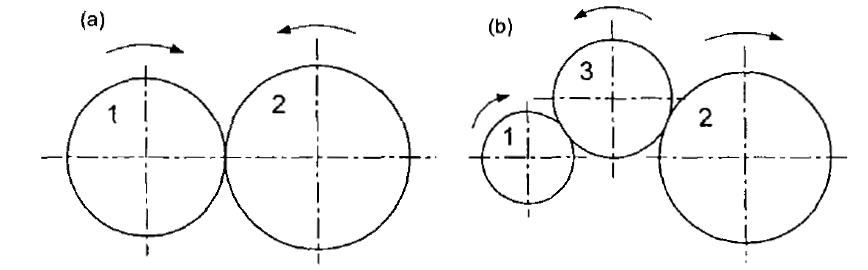
\includegraphics[width=4in]{engranes.jpg}
\caption{Tren de engranes simples}
\label{fig1}
\end{figure}

El signo negativo indica que los engranes $1$ y $2$ giran en dirección contraria. El engrane $3$ no afecta la relación de engranes pero si determina la dirección en la que gira el engrane $2$. El cociente $\gamma = z_2/z_1$ se le llama relación de engranes.

\section{Eficiencia de un tren de engranes}

Teniendo en cuenta la fricción, la eficiencia de un tren de engranes es
\begin{equation}
\label{equ103}
\eta  =\frac{Potencia de Salida}{Potencia de entrada}= \frac{P_2}{P_1}
\end{equation}

Así,

\begin{equation}
\label{equ104}
\eta = \frac{P_2}{P_1} = \frac{T_2 (2 \pi n_2)}{T_1 (2 \pi n_1)}= \frac{T_2 n_2}{T_1 n_2}
\end{equation}

De acuerdo a la ecuación \ref{equ101} $n_1/n_2 = | N_1 / N_2 |$ de tal forma que la ecuación \ref{equ104} queda

\begin{equation}
\label{equ105}
\frac{T_2 n_2}{T_1 n_1} = \frac{T_2 z_1}{T_1 z_2}
\end{equation}

El torque en el engrane $1$

\begin{equation}
\label{equ106}
T_1 = T_2 \frac{z_1}{z_2} \frac{1}{\eta}
\end{equation}

\section{Momento de inercia equivalente}

En el tren simple mostrado en la figura \ref{fig1}a, sean $J_1$, $J_2$ igual a los momentos de inercia de las masas rotativas de los engranes $1$ y $2$, $\Omega _1$ y $\Omega _2$ es igual a la velocidad angular de los engranes $1$ y $2$, $D_1$ y $D_2$ es igual al diametro del círculo del engrane $1$ y $2$, $0.5 J_1 \Omega _1 ^2$, $0.5 J_2 \Omega _2^2$ es igual a la energía cinética de los engranes $1$ y $2$, respectivamente.
La energia neta suministrada a el sistema por unidad de tiempo es igual a la velocidad de cambio de la energía cinética $E_k$, i.e.

\begin{equation}
\label{equ107}
P = \frac{d E_k}{dt}= T \Omega _1
\end{equation}

Si sustituimos las energías cinéticas de los engranes y la igualamos a la energía mecánica suministrada por el motor obtenemos,

\begin{equation}
\label{equ108}
\begin{aligned}
T \Omega_{1} & = \frac{d}{d t} [\frac{1}{2} J_1 \Omega _1 ^2 + \frac{1}{2} J_2 \Omega _2 ^2]\\
 & =\frac{1}{2} (J_1 + \frac{\Omega _2 ^2}{\Omega _1 ^2}J_2) \frac{d}{d t}\Omega _1^2 \\
& = \frac{1}{2} (J_1 + \frac{\Omega _2^2}{\Omega _1^2} J_2) 2 \Omega _1 \frac{d \Omega _1}{d t}
\end{aligned}
\end{equation}

La cantidad $J_1 + (\Omega _2 / \Omega _1)^2 J_2$ se puede denominar como el momento de inercia equivalente de los engranes respecto de la rueda $1$ (o engrane $1$). Los momentos de inercia de varios engranes pueden ser reducidos a un momento de inercia equivalente en la flecha del motor, i.e.

\begin{equation}
\label{equ109}
T=  (J_1 + \frac{\Omega _2^2}{\Omega _1^2} J_2) \frac{d \Omega _1}{d t}=(J_1 + \frac{z_1^2}{z_2^2} J_2) \frac{d \Omega _1}{d t}
\end{equation}

El momento de inercia equivalente es igual a el momento de inercia de cada rueda en el tren multiplicada por el cuadrado de su razon de engranes respecto de la rueda de referencia.

\section{Características mecánicas de máquinas}

En general, las características mecánicas de una maquina $T= f(\Omega)$ manejada por un motor eléctrico se puede describir por la siguiente ecuación:

\begin{equation}
\label{equ110}
T = T_r \left ( \frac{\Omega}{\Omega _r} \right ) ^\beta
\end{equation}

donde $T_r$ es el torque de resistencia de la maquina a la velocidad angular $\Omega _r$, $\beta =0$  para montacargas, cintas transportadoras, máquinas rotativas, y vehículos (máquina de torque constante), $\beta =1$ para molinos, máquinas de papel, máquinas textiles, $\beta = 2$ para bombas rotatorias, ventiladores, turbocompresores y sopladores.

\section{Ecuación de balance de torque}

Un sistema electromecánico se puede describir con la ayuda de la siguiente ecuación de balance de torque
\begin{equation}
\label{equ111}
J \frac{d ^2 \theta}{d t ^2}+ D \frac{d \theta}{d t}+ K \theta = T_d \mp T_{sh}
\end{equation}
donde $J$ es el momento de inercia del sistema en $kg m^2$ la cual se supone constante ($d J / dt =0$), $D$ es el coeficiente de amortiguamiento en $N s/ m$, $K$ es el coeficiente de rigidez o constante del resorte en $N/m$, $T_d$  es el torque electromagnetico instantaneo del motor, $T_{sh}$ es el torque de carga instantaneo (flecha), $\theta$ es el ángulo de desplazamiento, el signo "$-$" es para aceleración (modo motor), y el signo "$+$" es para la desaceleración (modo frenado).

Suponiendo $D=0$ y $K=0$ la ecuación de balance de torque queda

\begin{equation}
\label{equ112}
J \frac{d ^2 \theta}{d t^2} \approx T_d \mp T_{sh}
\end{equation}

\section{Ejemplo 1: Análisis del torque de maquinarias}

\begin{figure}
\centering
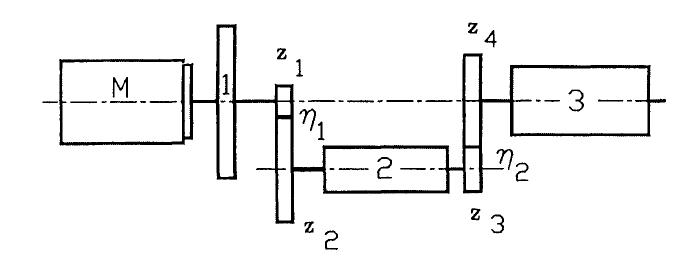
\includegraphics[width=4in]{trendelaminado.jpg}
\caption{Motor Eléctrico manejando un tren de laminado}
\label{fig2}
\end{figure}

Encontrar el torque de estado estable, potencia de salida, y momento de inercia de un motor eléctrico impulsando un tren de laminado como se muestra en la figura \ref{fig2}. La velocidad del motor es $n=730 rpm$. El volante de inercia y los rodillos estan hechos de acero con densidad de masa específica $\rho = 7800 kg/m^3$.

El volante de inercia sólido 1: diametro $D_1=1.5m$, grosor $l_1=0.2 m$

Primer rodillo 2: diametro $D_2=0.4m$, longitud $l_2=0.8m$, fuerza periférica $F_2=20kN$, número de dientes del primer engrane $z_1=15$, $z_2=35$, eficiencia del primer engrane $\eta_1=0.87$.

Segundo rodillo 3: diametro $D_3=0.5m$, longitud $l_3=1.2m$, fuerza periférica $F_3=14kN$, número de dientes del primer engrane $z_3=20$, $z_4=45$, eficiencia del primer engrane $\eta_1=0.9$.

\subsection{Solución}

El torque de la flecha (carga) en base a la ecuación \ref{equ106}

\begin{equation}
\label{equ113}
T_{sh}= F_2 \frac{D_2}{2}\frac{z_1}{z_2}\frac{1}{\eta _1}+F_3\frac{D_3}{2}\frac{z_1}{z_2}\frac{z_3}{z_4}\frac{1}{\eta _1}\frac{1}{\eta _2}=2.82 kNm
\end{equation}

en donde la relación de engranes es $z_2/z_1$.

La salida de potencia del motor
\begin{equation}
\label{equ114}
P_{out}=2 \pi n T_{sh}= 2 \pi (\frac{730}{60}) 2820=216 kW
\end{equation}

La masa del volante de inercia

\begin{equation}
\label{equ115}
m_1=\rho \frac{\pi D_1^2}{4}l_1=2757 kg
\end{equation}

La masa del primer rodillo

\begin{equation}
\label{equ116}
m_2=\rho \frac{\pi D_2^2}{4}l_2=785 kg
\end{equation}

La masa del segundo rodillo

\begin{equation}
\label{equ117}
m_3=\rho \frac{\pi D_3^2}{4}l_3=1840 kg
\end{equation}

El momento de inercia del volante de inercia
\begin{equation}
\label{equ118}
J_1 = m_1 \frac{D_1^2}{8}= 776 kgm^2
\end{equation}

El momento de inercia del primer rodillo
\begin{equation}
\label{equ119}
J_2 = m_2 \frac{D_2^2}{8}= 15.7 kgm^2
\end{equation}

El momento de inercia del segundo rodillo
\begin{equation}
\label{equ120}
J_3 = m_3 \frac{D_3^2}{8}= 57.5 kgm^2
\end{equation}

El momento de inercia total del sistema respecto a la flecha del motor se obtiene

\begin{equation}
\label{equ121}
J= J_1+J_2 (\frac{z_1}{z_2})^2+J_3 (\frac{z_1 z_3}{z_2 z_4})= 781 kgm^2
\end{equation}

\section{Ejemplo 2}

Un motor eléctrico de 12 kW, 1000 rpm trabaja a velocidad casi constante de acuerdo con el perfil de torque dado en la figura \ref{fig3}. La capacidad de sobrecarga tiene un factor $k_{ocf}=T_{max}/T_{shr}=2$. Encontrar el coeficiente de utilización térmica del motor.

\begin{figure}
\centering
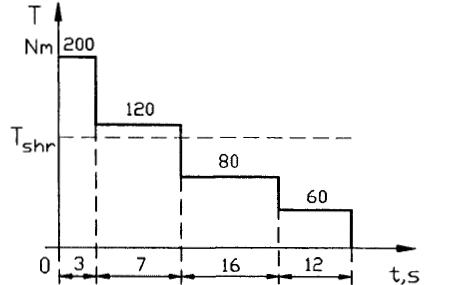
\includegraphics[width=4in]{perfildetorque.jpg}
\caption{Perfiles de torque para el ejemplo 2}
\label{fig3}
\end{figure}

\subsection{Solución}

El torque requerido en la flecha se calcula

\begin{equation}
\label{equ122}
T_{shr}=\frac{P_{out}}{2 \pi n}=\frac{12000}{2 \pi (1000/60)}=114.6 Nm
\end{equation}

El torque $rms$ basado en el ciclo de trabajo

\begin{equation*}
T_{rms}^2 (t_1+t_2+t_3+...+t_n)  =(T_1^2 t_1+T_2^2 t_2+T_3^2 t_3+...+T_n^2 t_n)
\end{equation*}

\begin{equation*}
T_{rms} \sum_{l=1}^{n} t_l = \sum_{i=1}^{n} T_i t_i
\end{equation*}

\begin{equation}
\label{equ123}
 T_{rms}  = \sqrt{\frac{\sum_{i=1}^{n} T_i t_i}{ \sum_{l=1}^{n} t_l}}
\end{equation}

Tomando en cuenta los valores de la figura \ref{fig3} obtenemos

\begin{equation*}
 T_{rms}  = \sqrt{\frac{(200^2) 3+(120^2) 7 + (80^2) 16 + (60^2) 12 }{ 3+7+16+12}}= 95.5 Nm
\end{equation*}

El máximo torque en la figura \ref{fig3} no puede exceder el número de veces el factor de la sobre carga del torque nominal de la flecha $k_{ocf} T_{shr}$. Tambien, el torque $T_{shr}$  debe  ser mayor o igual que $T_{rms}$.

El coeficiente de utilización térmica del motor

\begin{equation*}
\frac{T_{rms}}{T_{sh}}100 \% = \frac{95.5}{114.6}100=83.3 \%
\end{equation*}

\section{Ejemplo numérico 3}

El torque requerido y el perfil de velocidad de un controlador de un servo estan mostrados en la figura. A velocidad constante 2500 rpm, el torque de la carga en la flecha es $T_{sh} = 1.5 Nm$. La inercia de la carga sometida a el eje del motor es $J_L = 0.004 kgm^2$. Suponiendo la inercia del servomotor $J_M = 0.5 J_L$, elegir un servomotor de imanes permanentes sin escobillas.

\begin{figure}
\centering
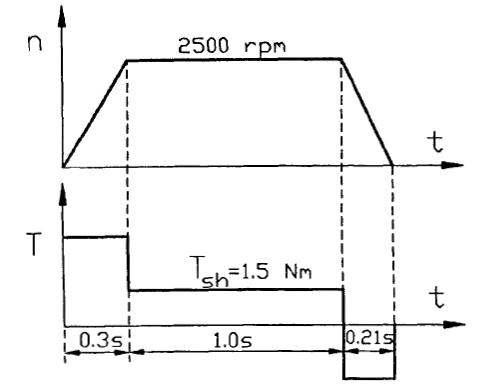
\includegraphics[width=4in]{perfilcarga.jpg}
\caption{Perfiles de carga para el ejemplo 3}
\label{fig4}
\end{figure}

\subsection{Solución}

El balance mecánico es expresado como


\begin{equation*}
2 \pi J \frac{\Delta n}{\Delta t} = T_d \pm T_{sh}
\end{equation*}

en donde $T_d$ es el torque electromagnético desarrollado por el motor para acelerar o frenar, el signo '$-$' es para la aceleración, y el signo '$+$' es para desaceleración.

El torque del motor necesario para la aceleración

\begin{equation*}
T_d = 2 \pi (J_M +J_L) \frac{\Delta n}{\Delta t}+T_{sh}=\frac{2 \pi}{60}(0.004+0.002) \frac{2500-0}{0.3-0}+1.5 \approx 6.74  Nm
\end{equation*}

El torque del motor requerido para frenado

\begin{equation*}
T_d = 2 \pi (J_M +J_L) \frac{\Delta n}{\Delta t}-T_{sh}=\frac{2 \pi}{60}(0.004+0.002) \frac{2500-0}{0.21-0}-1.5 \approx 5.98 Nm
\end{equation*}

El torque $rms$

\begin{equation*}
T_{rms}= \sqrt{\frac{(6.74^2)0.3+(1.5^2)1.0+(5.98^2)0.21 }{0.3+1.0+0.21 }} = 3.93 Nm
\end{equation*}

La potencia de salida calculada para el torque  $rms$

\begin{equation*}
P_{out}= T_{rms}(2 \pi n) = (3.93)(2 \pi) \frac{2500}{60} = 1030 W
\end{equation*}

El factor de sobrecarga para $T_{dmax}=6.74 Nm$

\begin{equation*}
\frac{T_{dmax}}{T_{rms}}= \frac{6.74}{3.93}=1.715
\end{equation*} 

Un motor de Imanes permanentes sin escobillas de 1.1 kW con un factor de capacidad de sobrecarga mínima de 1.8 es recomendada.

\section{Ejemplo numérico 4}

Un motor eléctrico de 10 kW, de 1450 rpm esta siendo usado para manejar las siguientes máquinas: (a) una grúa ($\beta =0$), (b) Un molino ($\beta = 1$) (c) un ventilador ($\beta =2$).  El torque de carga en cada caso en de 60 Nm. Encontrar la pérdida en la potencia mecánica si la velocidad es reducida a $n= 1200 rpm$.

\subsection{Solución}

La salida de potencia entregada por el motor a $T_r= 60 Nm$ y $n_r=1450 rpm$

\begin{equation*}
P_{outr}=T_r \Omega _r = T_r (2 \pi n_r) = 60 (2 \pi \frac{1450}{60}) = 9111 kW
 \end{equation*}

(a) para una grúa 

\begin{equation*}
T = 60 (\frac{1200}{1450})^0=60 Nm
\end{equation*}

\begin{equation*}
P_{out}=T(2 \pi n)=60 (2 \pi \frac{1200}{60})= 7540 W
\end{equation*}

(b) para el molino

\begin{equation*}
T = 60 (\frac{1200}{1450})^1=49.7 Nm
\end{equation*}

\begin{equation*}
P_{out}=T(2 \pi n)=49.7 (2 \pi \frac{1200}{60})= 6245 W
\end{equation*}

(c) para el ventilador

\begin{equation*}
T = 60 (\frac{1200}{1450})^2=41.1 Nm
\end{equation*}

\begin{equation*}
P_{out}=T(2 \pi n)=41.1 (2 \pi \frac{1200}{60})= 5165 W
\end{equation*}

La potencia mecánica a velocidad reducida y referenciada a la potencia nominal es

(a) para la grúa

\begin{equation*}
\frac{7540}{9111}100=82.7 \%
\end{equation*}

(b) para el molino

\begin{equation*}
\frac{6245}{9111}100=68.5 \%
\end{equation*}

(c) para el ventilador

\begin{equation*}
\frac{5165}{9111}100=56.7 \%
\end{equation*}

\chapter{Imanes Permanentes y circuitos}

Un iman permanente puede producir un campo magnético en el entrehierro sin necesidad de un campo de exitación y sin disipar potencia eléctrica. La energía externa es necesaria solamente para cargar la energía del campo magnético. no para mantenerlo. Como otro material ferromagnético, un iman permanente puede ser descrito por su ciclo de histéresis B-H. Los imanes permanentes son tambien llamados Materiales magnéticos duros, lo cual significa que son materiales ferromagnéticos con un ciclo de histéresis ancho. 

La base para la evaluación de un imán permanente es la porción de el ciclo de histéresis localizado en la parte superior del segundo cuadrante, llamado curva de demagnetización (\ref{fig304}). Si la intensidad de un campo magnético inverso es aplicado a uno previamente magnetizado, por decir, un especimén toroidal, la densidad de flujo magnético cae a una magnitud determinado por el punto $K$. Cuando la densidad de  flujo magnético se quita, la densidad de flujo regresa a el punto $L$ de acuerdo a el lazo de histéresis menor. Así, la aplicación de un campo inverso reduce el remanente, o magnetismo remanente. Reaplicando la intensidad de un campo magnético nuevamente reduce la densidad de flujo, completando el lazo menor de histéresis regresando el material al mismo valor de la densidad de flujo al punto $K$ como antes. El lazo de histéresis menor puede generalmente ser reemplazado con un pequeño error por una linea llamada línea de retroceso. Esta linea tiene un pendiente llamada la permeabilidad de retroceso $\mu_{rec}$.

\begin{figure}
\centering
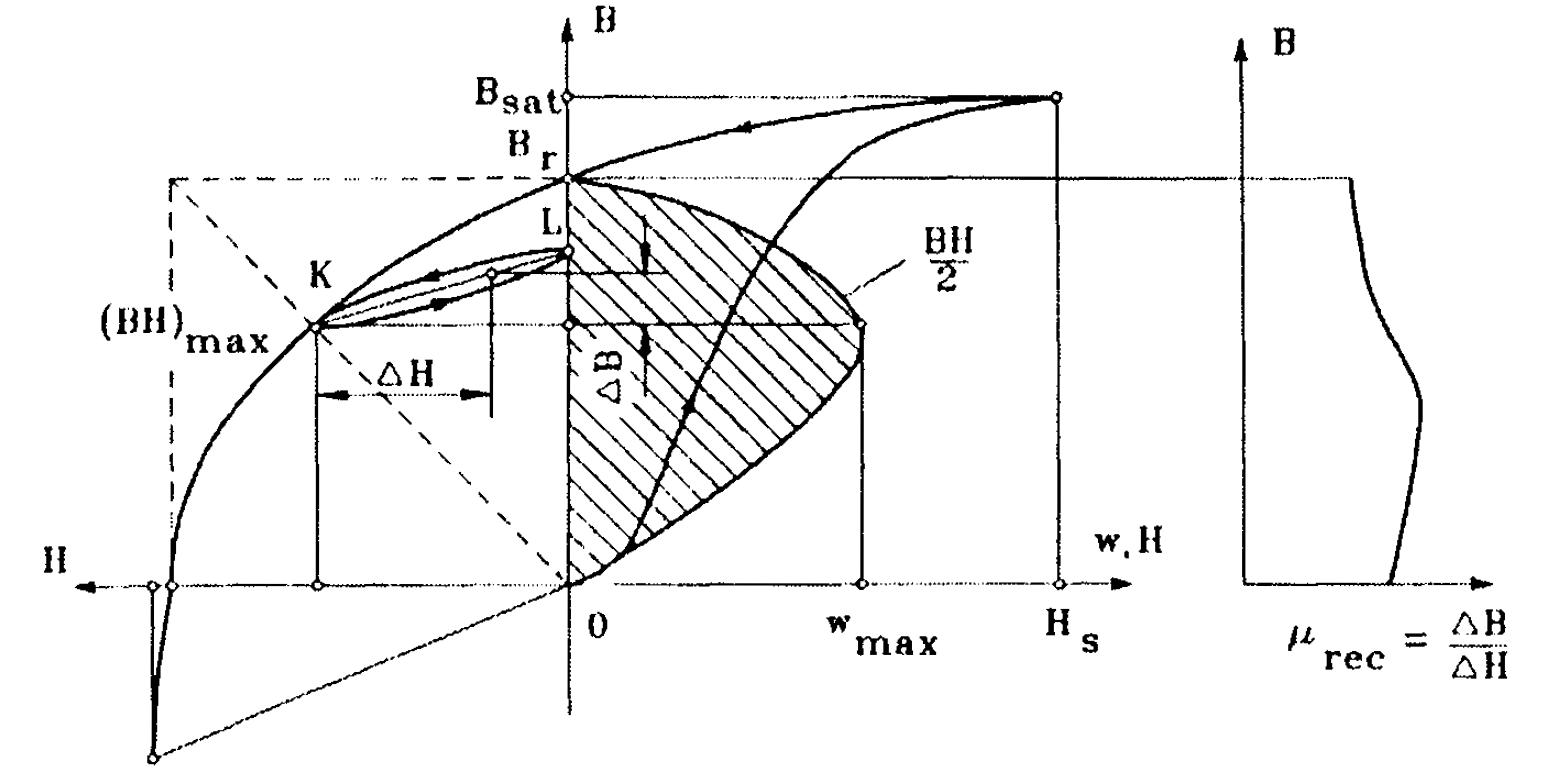
\includegraphics[width=5in]{demagne.jpg}
\caption{Curva de demagnetización, lazo de retroceso, energía de un Iman Permanente, y permeabilidad magnetica de retroceso }
\label{fig304}
\end{figure}

Siempre que el valor negativo de la intensidad de campo magnético aplicado no exceda el valor máximo correspondiente a el punto $K$, el imán permanente puede ser considerado razonablemente permanente. Si una intensidad de campo magnetico $H$  negativo mucho mayor es aplicado, la densidad de flujo magnético se reducirá a un valor inferior que el punto $K$. En la eliminación de $H$, un nuevo y menor linea de retoceso se establecerá.

La ecuación que relaciona la densidad de flujo de magnetización $B$, la magnetización intrínseca $B_i$ debido a la precensia de un material ferromagnético, y la intensidad de campo magnético $H$ puede ser expresada como

\begin{equation}
\label{equ300}
\vec{B} = \mu _0 \vec{H} + \vec{B_i} = \mu _0 (\vec{H}+\vec{M}) = \mu _0 (1+ \chi) \vec{H} = \mu _0 \mu _r \vec{H}
\end{equation}

en el cual $\vec{B}$, $\vec{H}$, $\vec{B_i}$ y $\vec{M}=\vec{B_i}/\mu _0$ son vectores paralelos o antiparalelos, asi la ecuación \ref{equ300} puede ser escrita en una forma escalar. La permeabilidad mágnetica del espacio libre es $\mu_0 = 0.4 \pi x 10^{-6}$ H/m. La permeabilidad magnética relativa de materiales ferromagnéticos es $\mu_r = 1+ \chi >>1$. EL vector de magnetización $\vec{M}$ es proporcional a la susptibilidad magnética del material $\chi$. La densidad de flujo $\mu_0 H$  estaría presente dentro un toroide si el núcleo ferromagnético no esta puesto. La densidad de flujo $B_i$ es la contibución del núcleo ferromagnético.

Un imán permanente es inenerentemente diferente que un electromagneto. Si un campo externo $H_a$ es aplicado al imán permanente, como fue necesario para obtener el lazo de histéresis de la figura \ref{equ300}, el campo magnético resultante es

\begin{equation}
\label{equ301}
\vec{H} = \vec{H_a}+ \vec{H_d}
\end{equation}

donde $-\vec{H_d}$ es un potencial existente entre los polos, 180 grados  opuestos a $B_i$, proporcional a la magnetización intrínseca $B_i$. En un circuito magnético cerrado, e.g. el toroide, la intensidad de campo magnético resultante desde la magnetización intrínseca $H_d=0$. Si el imán permanente es removido del circuito magnético

\begin{equation}
\label{equ302}
H_d = - \frac{M_b B_i}{\mu _0}
\end{equation}

donde $M_b$ es el coeficiente de damagnetización que depende de la geometría del material. Usualmente $M_b <1$. Estableciendo $B_i = B_d - \mu _0 H_d$ en la ecuación \ref{equ302} relacionando la densidad de flujo magnético $B_d$ y el campo de  autodemagnetización $H_d$ con la geometría del imán.

\begin{equation}
\label{equ303}
\frac{B_d}{\mu_0 H_d} = 1 - \frac{1}{M_b}
\end{equation}

El coeficiente ($1-1/M_b$) es porporcional a la permeabilidad del circuito magnetico externo.

Los imanes permanentes se caracterizan por los siguientes parámetros:

\begin{itemize}
\item Desidad de flujo magnético de saturación $B_{sat}$ y la intensidad de campo magnético de saturación $H_{sat}$. En este punto el alineamiento de todos los dominios de momentos magnéticos en la dirección del campo externo aplicado.

\item Densidad de flujo magnético remanente $B_r$, o remanencia, es la densidad de flujo magnético correspondiente a la intensidad de campo magnético de cero. Una alta remanencia significa que el imán puede soportar una densidad de flujo magnético más alta en el entrehierro del circuito magnético.

\item Intensidad de campo coercitivas $H_c$ o coercitividad, es el valor de la intensidad de  campo de demagnetización necesario para llevar la densidad de flujo magnético a cero en un material previamente magnetizado (en condiciones de magnetización ciclica y simétrica). Una alta coercitividad significa que, un magneto mas delgado puede ser usado para resistir el campo de demagnetización.

\item Curva de demagnetización intrínseca (fig \ref{fig304}) es una porción del lazo de histéresis  $B_i = f(H)$ localizado en la parte superior del segundo cuadrante, en donde $B_i=B-\ mu_0 H$ de acuerdo a la ecuación \ref{equ300}. Para $H=0$ la densidad de flujo intrínseco es $B_i=B_r$.

\item Coercitividad Intrínseca, ${}_i H_c$ es la intensidad de campo magnético necesaria para traer a cero la densidad de flujo magnético intrínseca $B_i$ de un amterial magnético descrito por la curva $B_i=f(H)$. para materiales ${}_{i}H_{c}> H_c$.

\item Permeabilidad magnética de retroceso, $\mu_{rec}$ es la razón de la densidad de flujo magnético sobre la intensidad de campo magnético en cualquier punto de la curva de demagnetización, i.e.,

\begin{equation}
\label{equ304}
\mu _{rec} = \mu _0 \mu_{rrec}= \frac{\Delta B}{\Delta H}
\end{equation}

donde la permeabilidad relativa de retroceso es $\mu _{rrec}=1...3.5$.

\item Energía magnética máxima por unidad producida por el imán permanente en el espacio externo es igual a  la densidad de energía magnética máxima por volumen, i.e.



\end{itemize} 



\chapter{Análisis de Energía}
Un análisis de potencia se utiliza para verificar la factibilidad de las especificaciones. La potencia necesaria para elevar un grado a una velocidad constante se analizará en primer lugar. La fuerza de arrastre es definido por la ecuación:
\begin{equation}
\label{equ200}
F_{arr}=\frac{1}{2} \rho C_d A v^2
\end{equation}

donde:

\begin{itemize}
\item $\rho = 2.33X10^{-3}  slug/ft^3$ (densidad del aire al nivel del mar)
\item $C_d=0.5$ (coeficiente de arrastre)
\item $A= 4X5$ pies (área frontal del carro)
\end{itemize}

Ahora, la fuerza debido a la pendiente se determina usando

\begin{equation}
\label{equ201}
F_{pendiente}= m g S_l
\end{equation}
donde $S_l$ es la pendiente. Y la fuerza debido a la resistencia de rodamiento es

\begin{equation}
\label{equ202}
F_{rod}= m g C_r
\end{equation}

donde: $C_r=0.01-0.015$ (coeficiente de rodamiento para llantas sobre concreto).
Ahora, la fuerza total se determina adicionando la fuerzas

\begin{equation}
\label{equ203}
F_{total}= F_{pendiente}+F_{rod}+F_{arr}
\end{equation}

Usando la fuerza calculada, la potencia se puede calcular usando la siguiente ecuación:

\begin{equation}
\label{equ204}
P=F_{total}v
\end{equation}


\backmatter
\end{document}
